% 2006 年全国卷Ⅱ理科第 19 题：直三棱柱
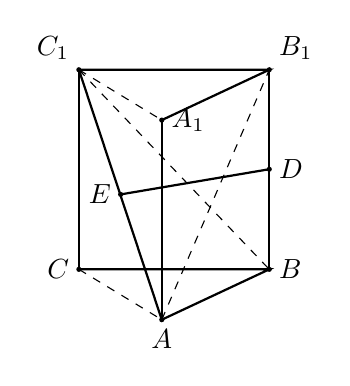
\begin{tikzpicture}[>=stealth,scale=0.78]
  \coordinate (A) at (2.20,0);
  \coordinate (B) at (3.95,0.82);
  \coordinate (C) at (0.85,0.82);
  \coordinate (A1) at (2.20,3.25);
  \coordinate (B1) at (3.95,4.07);
  \coordinate (C1) at (0.85,4.07);
  \coordinate (D) at (3.95,2.45);
  \coordinate (E) at (1.53,2.04);
  \draw[thick] (A)--(B)--(C);
  \draw[dashed] (C)--(A);
  \draw[thick] (A)--(A1) (B)--(B1) (C)--(C1);
  \draw[thick] (A1)--(B1)--(C1);
  \draw[dashed] (C1)--(A1);
  \draw[thick] (A)--(C1);
  \draw[dashed] (B)--(B1) (A)--(B1) (C1)--(B);
  \draw[thick] (D)--(E);
  \fill (A) circle (1.2pt) node[below] {$A$};
  \fill (B) circle (1.2pt) node[right] {$B$};
  \fill (C) circle (1.2pt) node[left] {$C$};
  \fill (A1) circle (1.2pt) node[right] {$A_1$};
  \fill (B1) circle (1.2pt) node[above right] {$B_1$};
  \fill (C1) circle (1.2pt) node[above left] {$C_1$};
  \fill (D) circle (1.2pt) node[right] {$D$};
  \fill (E) circle (1.2pt) node[left] {$E$};
\end{tikzpicture}
